\documentclass{classrep}
\usepackage[utf8]{inputenc}
\frenchspacing

\usepackage{graphicx}
\usepackage[usenames,dvipsnames]{color}
\usepackage[hidelinks]{hyperref}
\usepackage{lmodern}
\usepackage{placeins}
\usepackage{url}
\usepackage{amsmath, amssymb, mathtools}
\usepackage{listings}
\usepackage{fancyhdr, lastpage}
\usepackage{subfiles}

\pagestyle{fancyplain}
\fancyhf{}
\renewcommand{\headrulewidth}{0pt}
\cfoot{\thepage\ / \pageref*{LastPage}}

\definecolor{codegreen}{rgb}{0,0.6,0}
\definecolor{codegray}{rgb}{0.5,0.5,0.5}
\definecolor{codepurple}{rgb}{0.58,0,0.82}
\definecolor{backcolour}{rgb}{0.95,0.95,0.92}

\lstdefinestyle{mystyle}{
    commentstyle=\color{codegreen},
    keywordstyle=\color{magenta},
    numberstyle=\tiny\color{codegray},
    stringstyle=\color{codepurple},
    basicstyle=\ttfamily\footnotesize,
    breakatwhitespace=false,
    breaklines=true,
    captionpos=b,
    keepspaces=true,
    numbers=left,
    numbersep=5pt,
    showspaces=false,
    showstringspaces=false,
    showtabs=false,
    tabsize=2
}

\lstset{style=mystyle}

%--------------------------------------------------------------------------------------%
\studycycle{Informatyka stosowana, studia dzienne, II st.}
\coursesemester{II}

\coursename{Eksploracja danych internetowych}
\courseyear{2021/2022}

\courseteacher{dr inż. Kamil Stokfiszewski}
\coursegroup{poniedziałek, 12:15}

\author{%
    \studentinfo[239671@edu.p.lodz.pl]{Jan Karwowski}{239671}\\
    \studentinfo[239676@edu.p.lodz.pl]{Kamil Kowalewski}{239676}\\
}

\title{Zadanie 4.: Sieć neuronowa typu perceptron do kompresji obrazów}

\begin{document}
    \maketitle
    \thispagestyle{fancyplain}

    \tableofcontents
    \newpage

    \section{Cel} {
        Celem zadania było zaimplementowanie sieci typu autokoder do kompresji obrazów.
    }

    \section{Wstęp teoretyczny}
    \label{theoretical_intro} {
        Autokoder to perceptron wielowarstwowy, który składa się z neuronów liniowych z
        jedną warstwą ukrytą. Gdzie liczby neuronów w warstwie wejściowej i wyjściowej
        są takie same natomiast liczby neuronów w w warstwie ukrytej jej zazwyczaj
        mniejsza dzięki temu uzyskuje kompresje. Jest on wykorzystywany do kompresji
        danych lub ekstracji cech. Jego schemat został przedstawiony na rysunku
        \ref{autokoder}.

        \begin{figure}[!htbp]
            \centering
            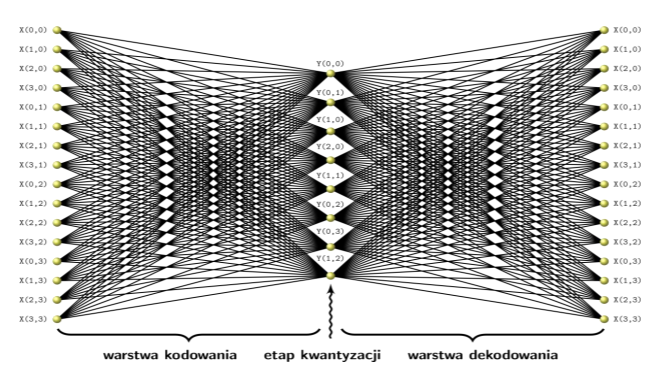
\includegraphics[width=\textwidth]{img/autokoder.png}
            \caption{Schemat sieci liniowej typu autokoder}
            \label{autokoder}
        \end{figure}
        \FloatBarrier

        W przypadku tego zadania zostały wykorzystane obrazy w formacie \textit{.bmp}
        o rozmiarze 512x512. Aby nie tworzyć wektora o liczbie wejść równej 512*512
        dokonuje sie operacji na mniejszych fragmentach np 8x8 co daje nam 8*8 neuronów
        na wejściu i wyjściu. Do oceny jakości obrazu po kompresji wykorzystywana jest
        miara \textit{PSNR}, której wzór został przedstawiony poniżej, wartość 512 nie
        jest przypadkowa gdyż jest ona brana z wielkości obrazu:

    % @formatter:off
        \begin{equation}
            PSNR = 10 \cdot \log_{10} \left(\frac{255^2}{\frac{1}{512^2}\sum_{i=0}^{511}\sum_{j=0}^{511}(x_ij - \hat{x}_ij)^2} \right)
        \end{equation}
    % @formatter:on

    }

    \section{Implementacja} {
        Autokoder został zaimplementowany w języku Python oraz takich bibliotek jak
        \textit{numpy} oraz \textit{Pillow} do operacji na obrazach. Do autokodera
        został wykorzystany \textit{MLPRegressor} z biblioteki \textit{sklearn}.

        Program zapewnia możliwość ustawienia następujących parametrów:
        \begin{itemize}
            \item Liczba neuronów w warstwie ukrytej \textbf{(--neurons\_sequence)}
            \item Liczba iteracji \textbf{(--iterations)}
            \item Współczynnik uczenia \textbf{(--learning\_rate)}
            \item Liczba wzorców treningowych \textbf{(--patterns\_number)}
            \item Szerokość wzorca \textbf{(--pattern\_width)} - jest to szerokość
            (a za razem długość bo to kwadrat) fragmentu obrazu, który został omówiony w
            sekcji \ref{theoretical_intro}. Parametr ten wskazuję też liczbę neuronów w
            warstwie wejściowej i wyjściowej.
            \item Ścieżki do obrazów treningowych \textbf{(--training\_images)}
        \end{itemize}
    }

    \section{Eksperymenty i wyniki} {
        \subsection{Opis eksperymentów} {
            \subfile{section/results_intro.tex}
        }
        \clearpage

        \subsection{Eksperyment nr 1}
        \label{exper_1} {
            \subfile{section/results_1.tex}
        }
        \clearpage

        \subsection{Eksperyment nr 2}
        \label{exper_2} {
            \subfile{section/results_2.tex}
        }
        \clearpage

        \subsection{Eksperyment nr 3}
        \label{exper_3} {
            \subfile{section/results_3.tex}
        }
        \clearpage

        \subsection{Eksperyment nr 4}
        \label{exper_4} {
            \subfile{section/results_4.tex}
        }
    }

    \section{Dyskusja} {
        Analizując uzyskane wartości PSNR, które zostały przestawione na wykresach można
        stwierdzić, że wyniki są z grubsza zbliżone do siebie. Oczywiście nie trudno
        zauważyć ciekawą rzecz na wykresie w sekcji \ref{exper_4}, że dla obrazu
        \textit{07.bmp} udało się uzyskać wartość powyżej 30 gdzie w innych przypadkach
        nie było to możliwe. Samo porównanie wyników nie jest sprawą oczywistą i
        trywialną gdyż każdy z eksperymentów zawierał inny zbiór treningowy a co za tym
        idzie inny zbiór testowy więc można mylnie pomyśleć, że w sekcji \ref{exper_2}
        udało się poprawic wyniki jednak nie jest to prawdą gdyż w zbiorze testowym nie
        ma obrazu \textit{02.bmp}.

        W żadnym przypadku nie udało się uzyskać wartości PSNR powyżej 40 więc człowiek
        może je odróżnić od oryginału. Różne zbiory treningowy miały wpływ na wyniki
        jednak różnice nie były ogromne. MLP wykorzystany w zadaniu potrzebuje dużej
        liczby wzorców oraz wielu iteracji aby dokonywać kompresji obrazów z
        zadawalającym efektem.
    }

    \begin{thebibliography}{0}
        % @formatter:off
        \bibitem{instrukcja}{Instrukcja do zadania, URL: https://ftims.edu.p.lodz.pl/pluginfile.php/151572/
        mod\_resource/content/1/perceptron\_kompresja\_obrazow.pdf}
        % @formatter:on
    \end{thebibliography}

\end{document}
